
\fullcite{daws16}

\begin{multicols}{2}
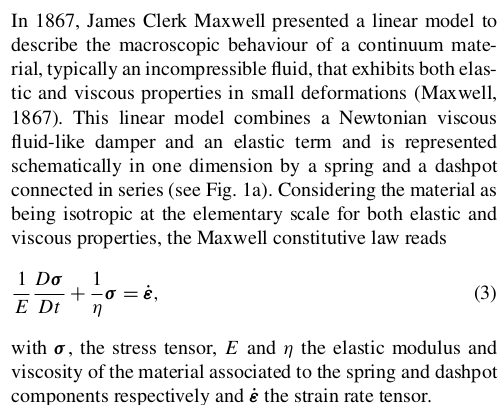
\includegraphics[width=8.25cm]{images/viscoelasticity/daws16a}\\
\[
\frac{1}{E} \frac{D{\bm \sigma}}{Dt} + \frac{1}{\eta} {\bm \sigma} = \dot{\bm\varepsilon}
\]
in 1d ?
\end{multicols}

\begin{multicols}{2}
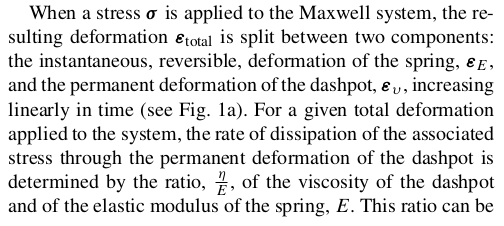
\includegraphics[width=8.25cm]{images/viscoelasticity/daws16b}
\end{multicols}

\begin{multicols}{2}
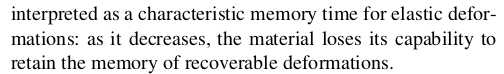
\includegraphics[width=8.25cm]{images/viscoelasticity/daws16c}
\end{multicols}

\begin{multicols}{2}
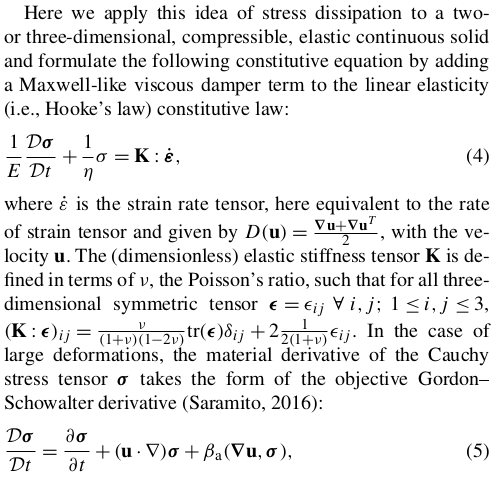
\includegraphics[width=8.25cm]{images/viscoelasticity/daws16f}\\
\[
\frac{1}{E} \frac{D{\bm \sigma}}{D t} + \frac{1}{\eta} \sigma 
= {\cal C}: \dot{\bm \varepsilon}
\]
with
\[
{\cal C}: \dot{\bm \varepsilon}
= \frac{\nu}{(1+\nu)(1-2\nu)} {\rm tr}({\bm \varepsilon}) {\bm 1}
+ 2\frac{1}{2(1+\nu)} {\bm \varepsilon}
\]

Gordon-Schowalter derivative:
\[
\frac{D{\bm \sigma}}{D t} = \frac{\partial{\bm \sigma}}{\partial t}
+ (\vec\upnu \cdot \vec\nabla) {\bm \sigma} +
\beta_a (\vec\nabla\vec\upnu,{\bm \sigma})
\]

\end{multicols}

\newpage

\begin{multicols}{2}
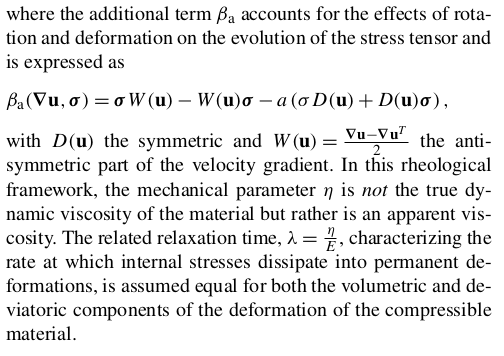
\includegraphics[width=8.25cm]{images/viscoelasticity/daws16d} \\
\[
\beta_a (\vec\nabla\vec\upnu,{\bm \sigma})
= {\bm \sigma}\cdot \dot{\bm \omega} - \dot{\bm \omega}\cdot {\bm \sigma}
- a ( {\bm \sigma} \cdot \dot{\bm \varepsilon}
+ \dot{\bm \varepsilon} \cdot {\bm \sigma})
\]
\end{multicols}



\begin{center}
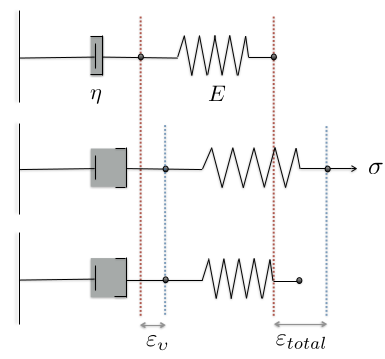
\includegraphics[width=8.25cm]{images/viscoelasticity/daws16e}\\
{\captionfont 
Schematic representations of the Maxwell model for a continuum material with 
elastic (shear) modulus $E$ and viscosity $\eta$. At time $t$, a stress is applied 
on the system. It is removed at time $t+\Delta t$: the spring goes back to its 
initial position but the dashpot retains its deformation $\varepsilon_v$.}
\end{center}













